\subsection{Multithreaded Kalman Filter Algorithm Proof of Concept} \label{ssec:prop_multithreaded_kf}

    \begin{wrapfigure}{r}{0.51\textwidth}
        \centering
        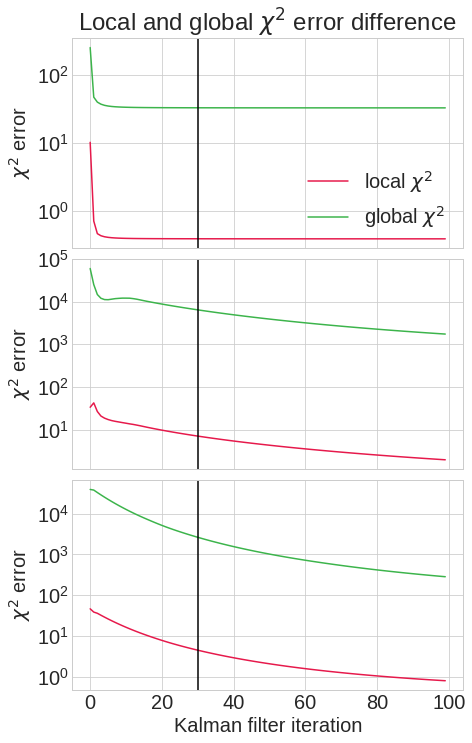
\includegraphics[width=1\textwidth]{multithreaded_kf/chi2error}
        \caption{\label{fig:mkf_chi2error} Local and global $\chi^2$ errors for a track in events \#$5$, \#$67$ and \#$103$ for $100$ KF iterations. The $30$ KF iterations commonly computed are marked by a black vertical line.}
    \end{wrapfigure}

A multithreaded Extended Kalman Filter (EKF) variant is proposed to accelerate the computation of the EKF in the code and to potentially obtain better solutions.
To understand why this option is deemed useful, it has to be noted that the EKF implementation described in Section \ref{ssec:framework_tf} contains a hardcoded stopping point for the EKF after $30$ iterations, with no dynamic analysis onto how good the solution found up to that point is or if the methods used have already converged.
Changing this might open the possibility of a multithreaded algorithm.

% DYNAMIC STOPPING POINT
Due to this, the first efforts were placed on finding this dynamic stopping point for the algorithm.
Naturally, this criteria must be related to the $\chi^2$ error, which is the variable that is being minimized by the method.
As mentioned before, a deifnition of the $\chi^2$ error is given in Appendix \ref{add:errors}.

The problem with this approach is that for every iteration of the EKF only the so-called ``local'' $\chi^2$ error is computed, while the ``global'' one is only computed once the EKF has finished.

% Note: if it's too hard to understand the local and global $\chi^2$ error then it might be better to leave this out for good.
The local $\chi^2$ error is computed while the EKF is running by projecting the state vector at a measurement site into the measurement itself and computing the squared difference divided by the uncertainty of the measurement.
The problem with this version of the error is that as the EKF runs, each state vector changes, and thus the error computed is different from the real one.

The global $\chi^2$ error is this ``real'' one, where each state vector near a measurement site is projected into it and the error is calculated.
The reason that the global error is only computed after the EKF has ran is that the process of updating the state vector across the particle trajectory is computationally-intensive, and thus doing it for each iteration of the EKF would be too expensive for the total computing time.

The problem that arises from this concept is that there are tracks where the convergence of the local $\chi^2$ error is not representative of the converge of the global one.
As can be seen in the first EKF iterations in the track from event \#$67$ in figure \ref{fig:mkf_chi2error}, the local and the global $\chi^2$ errors are not always correlated. % Note: I should find events where this lack of correlation is more apparent.

    \begin{figure}[ht]
        \centering
        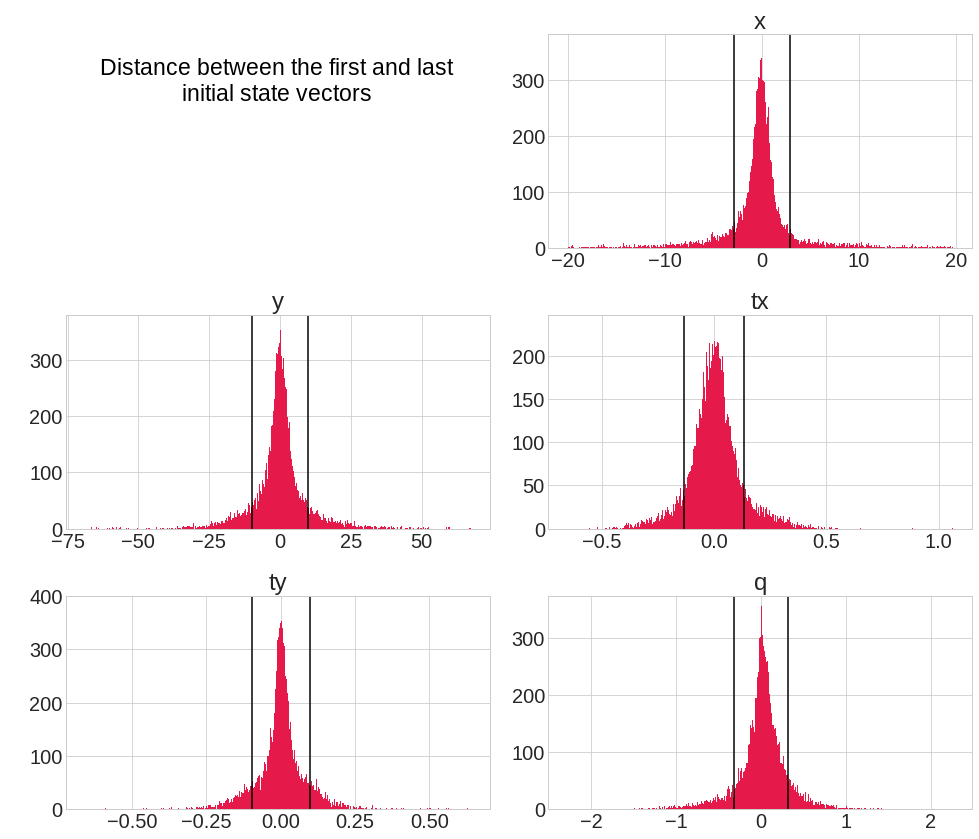
\includegraphics[scale=0.44]{multithreaded_kf/isv_distance}
        \caption{\label{fig:mkf_isv_distance} Distance between the first and the last initial vectors for the tracks found in $10.000$ events. The black lines mark a region where $80\%$ of the distances are contained.}
    \end{figure}

Then, the idea of computing different initial state vectors $\mathbf{x}(z) = \left<x, y, \theta_x, \theta_y, q\right>$ in parallel for each track was considered.
These different initial state vectors should be consistent, and this is pursued by comparing the different variables from the first and the last state vectors used by the Kalman filter.
This difference is recorded for all the tracks found in $10.000$ events and its distribution is evaluated.
A plot of this distribution for each variable in the state vector can be seen in Figure \ref{fig:mkf_isv_distance}.

    \begin{wrapfigure}{r}{0.51\textwidth}
        \centering
        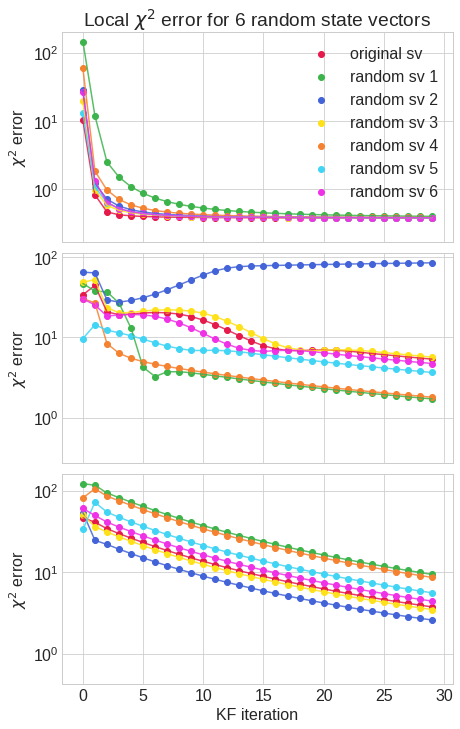
\includegraphics[width=1\textwidth]{multithreaded_kf/mkf_test}
        \caption{\label{fig:mkf_test} Local $\chi^2$ errors starting from $6$ random initial state vectors compared with the original in events \#$5$, \#$67$ and \#$103$ for $30$ KF iterations.}
    \end{wrapfigure}

To generate the initial state vector for the KF to run, a random perturbation inside a range that captures $80\%$ of the distance values (denoted as black vertical lines in Figure \ref{fig:mkf_isv_distance}) is added to the initial state vector and multiple instances of the KF are ran with these different initial state vectors. The resulting $\chi^2$ error obtained by running the KF in this manner for $6$ random initial state vectors can be seen in Figure \ref{fig:mkf_test}.

As can be seen in the figure, for the tracks in events $67$ and $103$ the final $\chi^2$ obtained from a random initial state vector was better than the one obtained for the original.
Special attention should be given to the ones obtained by the random state vectors $1$ and $4$ from event $67$ which are close to a fifth of the original one found.

% INCREASED POWER CONSUMPTION
It's worth noting that if a dynamic stopping point is implemented, that is to say, a point in which the KF is stopped before reaching the $30$ iterations, the multithreaded algorithm may provide better results in the same amount of time as the original one.

It's worth noting that while this algorithm may be able to provide better results in the same amount of time, the approach actually increases the total CPU-time and power consumption required to run the software.
This is due to the fact that multiple instances of the KF run in parallel.
In the case of the CLAS12 software as is ran in JLab, this additional power consumption meant that the algorithm was programmed but not implemented in the code due to power constraints.